%% Background
\chapter{Background}
\label{chap:background}

\section{Font Selection}

Surprisingly little progress has been made in the past several decades on the issue of user font selection. When a user searches for a new font, almost every major word processor presents them with the same interface: a basic, linear list of typefaces with a few controls over additional parameters like size, weight, and underline. This interface—essentially the same interface as was used by the earliest multi-font word processors—offers users very little support or guidance when traversing the growing number of unique fonts available to them.

% from Designing the Xerox “Star” User Interface, Byte, issue 4, 1982
\begin{figure}[h]
    \centering
    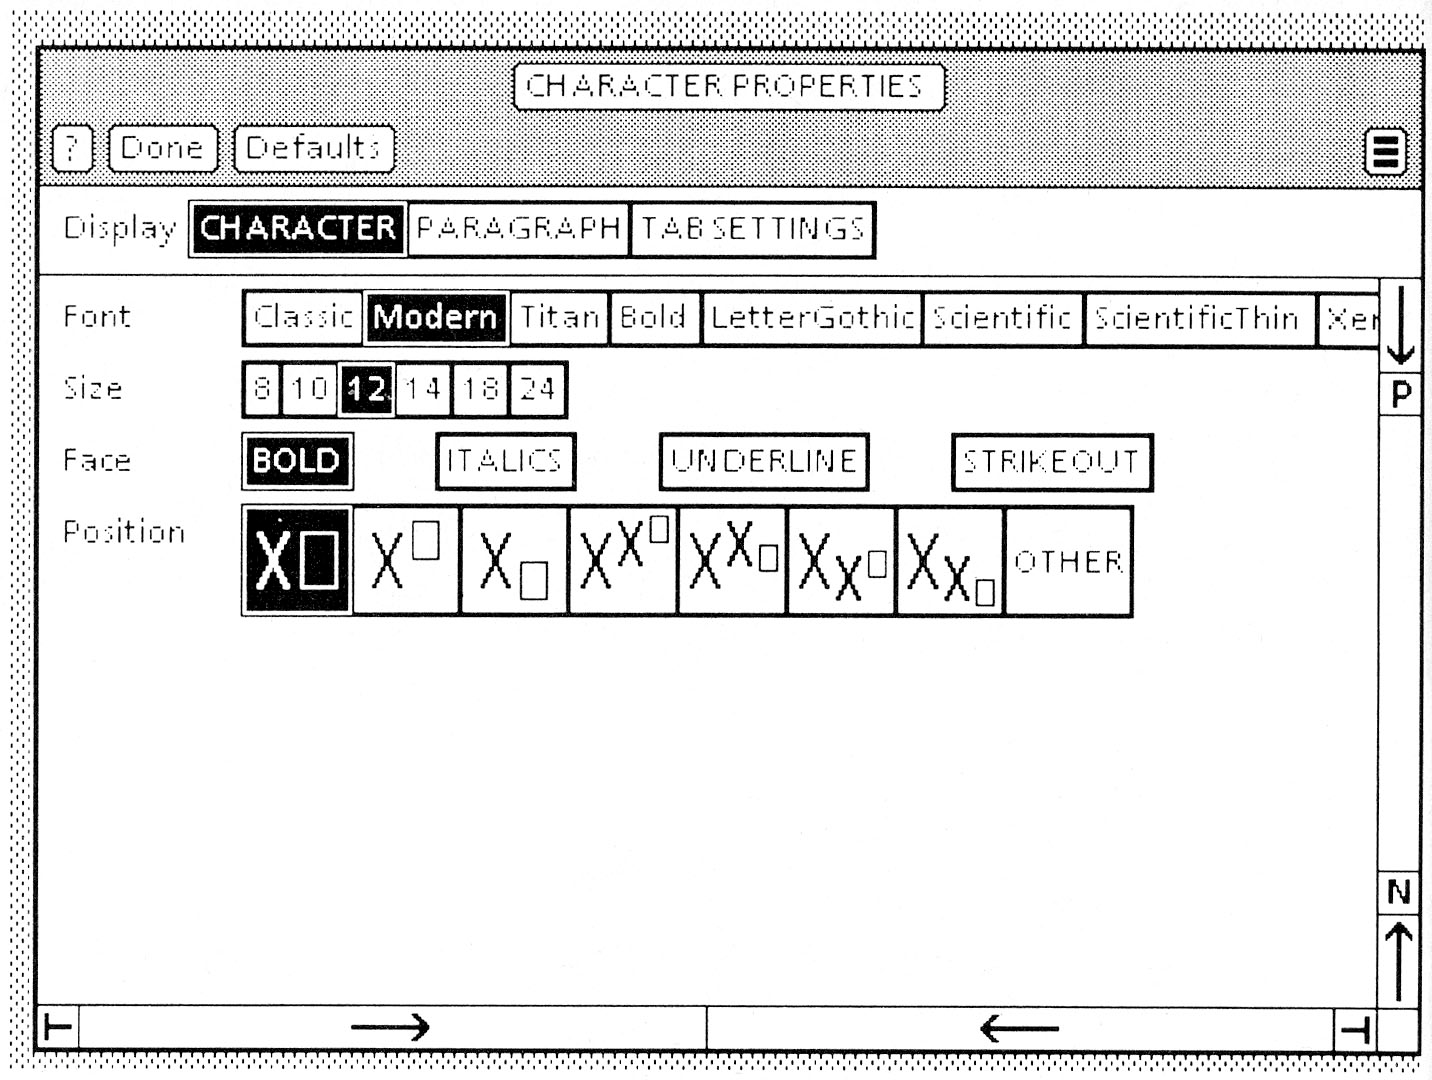
\includegraphics[width=.8\textwidth]{images/xerox-star.png}
    \caption{Font selection interface in Xerox Star (1981).}
    \label{fig:xerox-star}
\end{figure}

% own screenshots
\begin{figure}[h]
    \centering
    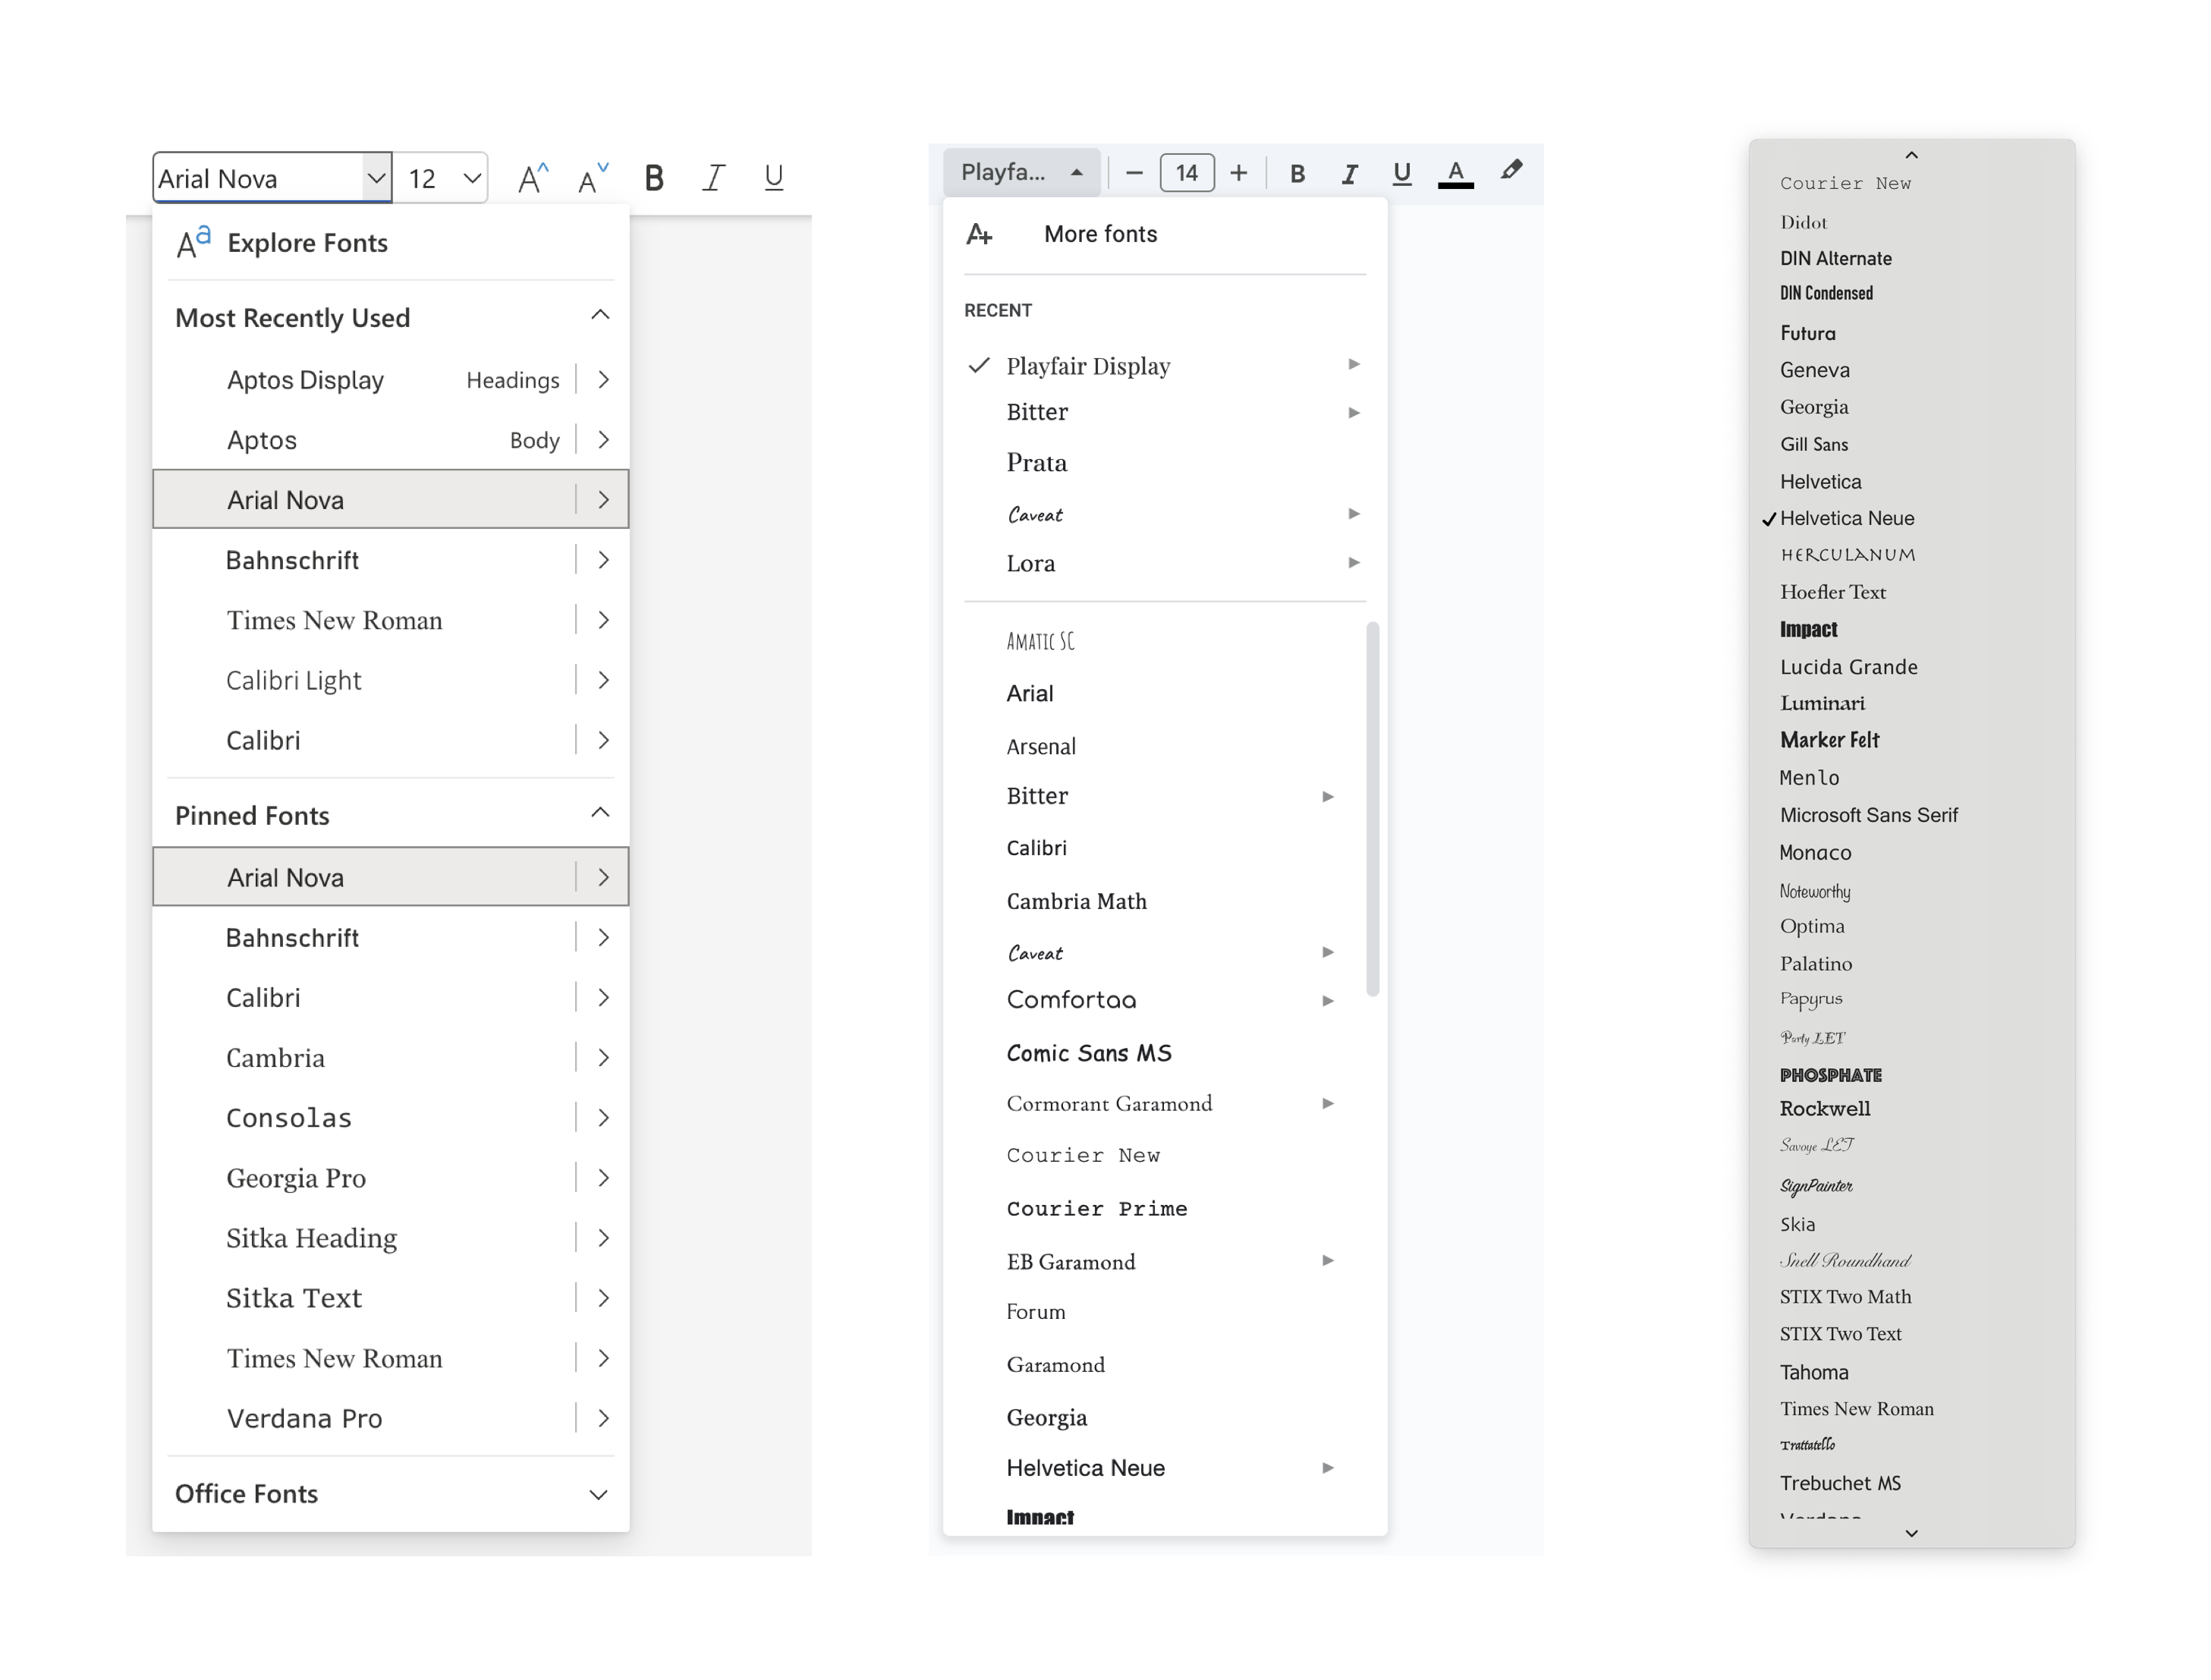
\includegraphics[width=1\textwidth]{images/font-selectors.png}
    \caption{Current font selection interfaces in Microsoft Word, Google Docs, and Apple Pages.}
    \label{fig:font-selectors}
\end{figure}

O'Donovan et al. list several reasons for the difficulty of developing font selection tools. The first issue is the sheer number of available fonts \cite{odonovan2014}. ``Most computers are now equipped with hundreds of fonts,'' they note, while online resources provide access to hundreds of thousands. Another issue is that there are not obvious ways to categorize fonts which correspond to a user's goal. While there exist broad categories like Serif, Sans Serif, and Handwritten, these must be manually designated on a per-font basis, and they do not necessarily categorize fonts along the lines which would be helpful for a user. A coffee shop owner deciding on a font for their shop's logo, for example, might not find the distinction between Serif and Sans Serif particularly useful, or know where to start in deciding between them. A graphic designer, who has studied design for years and has relevant experience, might feel confident in handling these decisions, but the typical user of a font selection tool does not have the tools, given the current font selector landscape, to make one of the most fundamental decisions to effective text-based graphical design. Finally, different users' goals in font selection vary. One user may be looking to match a particular font they found on a store sign, or to find a close match to a commercial font which is free to use. Another may be looking to match a particular mood, or choose a font that fits well with the rest of their document. A third may simply be exploring a large set of fonts like Adobe TypeKit or Google Fonts. O'Donovan et al. argues—and I agree—that current methods of font selection fall short on these issues and many more. Given the large number of fonts available to the modern user, a linear list of fonts is an  unrealistic and unhelpful tool.

Based on these issues, O'Donovan et al. presents three novel interfaces for font selection: one based on verbal attributes such as ``formal,'' ``friendly,'' or ``legible'' (Attribute Interface); another which clusters fonts hierarchically based on visual similarity (Group Interface); and a third, to be paired with the other two methods, which provides users with a list of similar font to the current selection (Search-By-Similarity). The researchers build these models on crowdsourced data collected through Amazon's Mechanical Turk with questions like ``Which of these two fonts is stronger?'', and they evaluated the interfaces using various design tasks on Mechanical Turk as well. Participants were three times more likely to succeed in a font-matching task, for example, using the Group Interface than the baseline font selector tool.

% own screenshots
\begin{figure}[h]
    \centering
    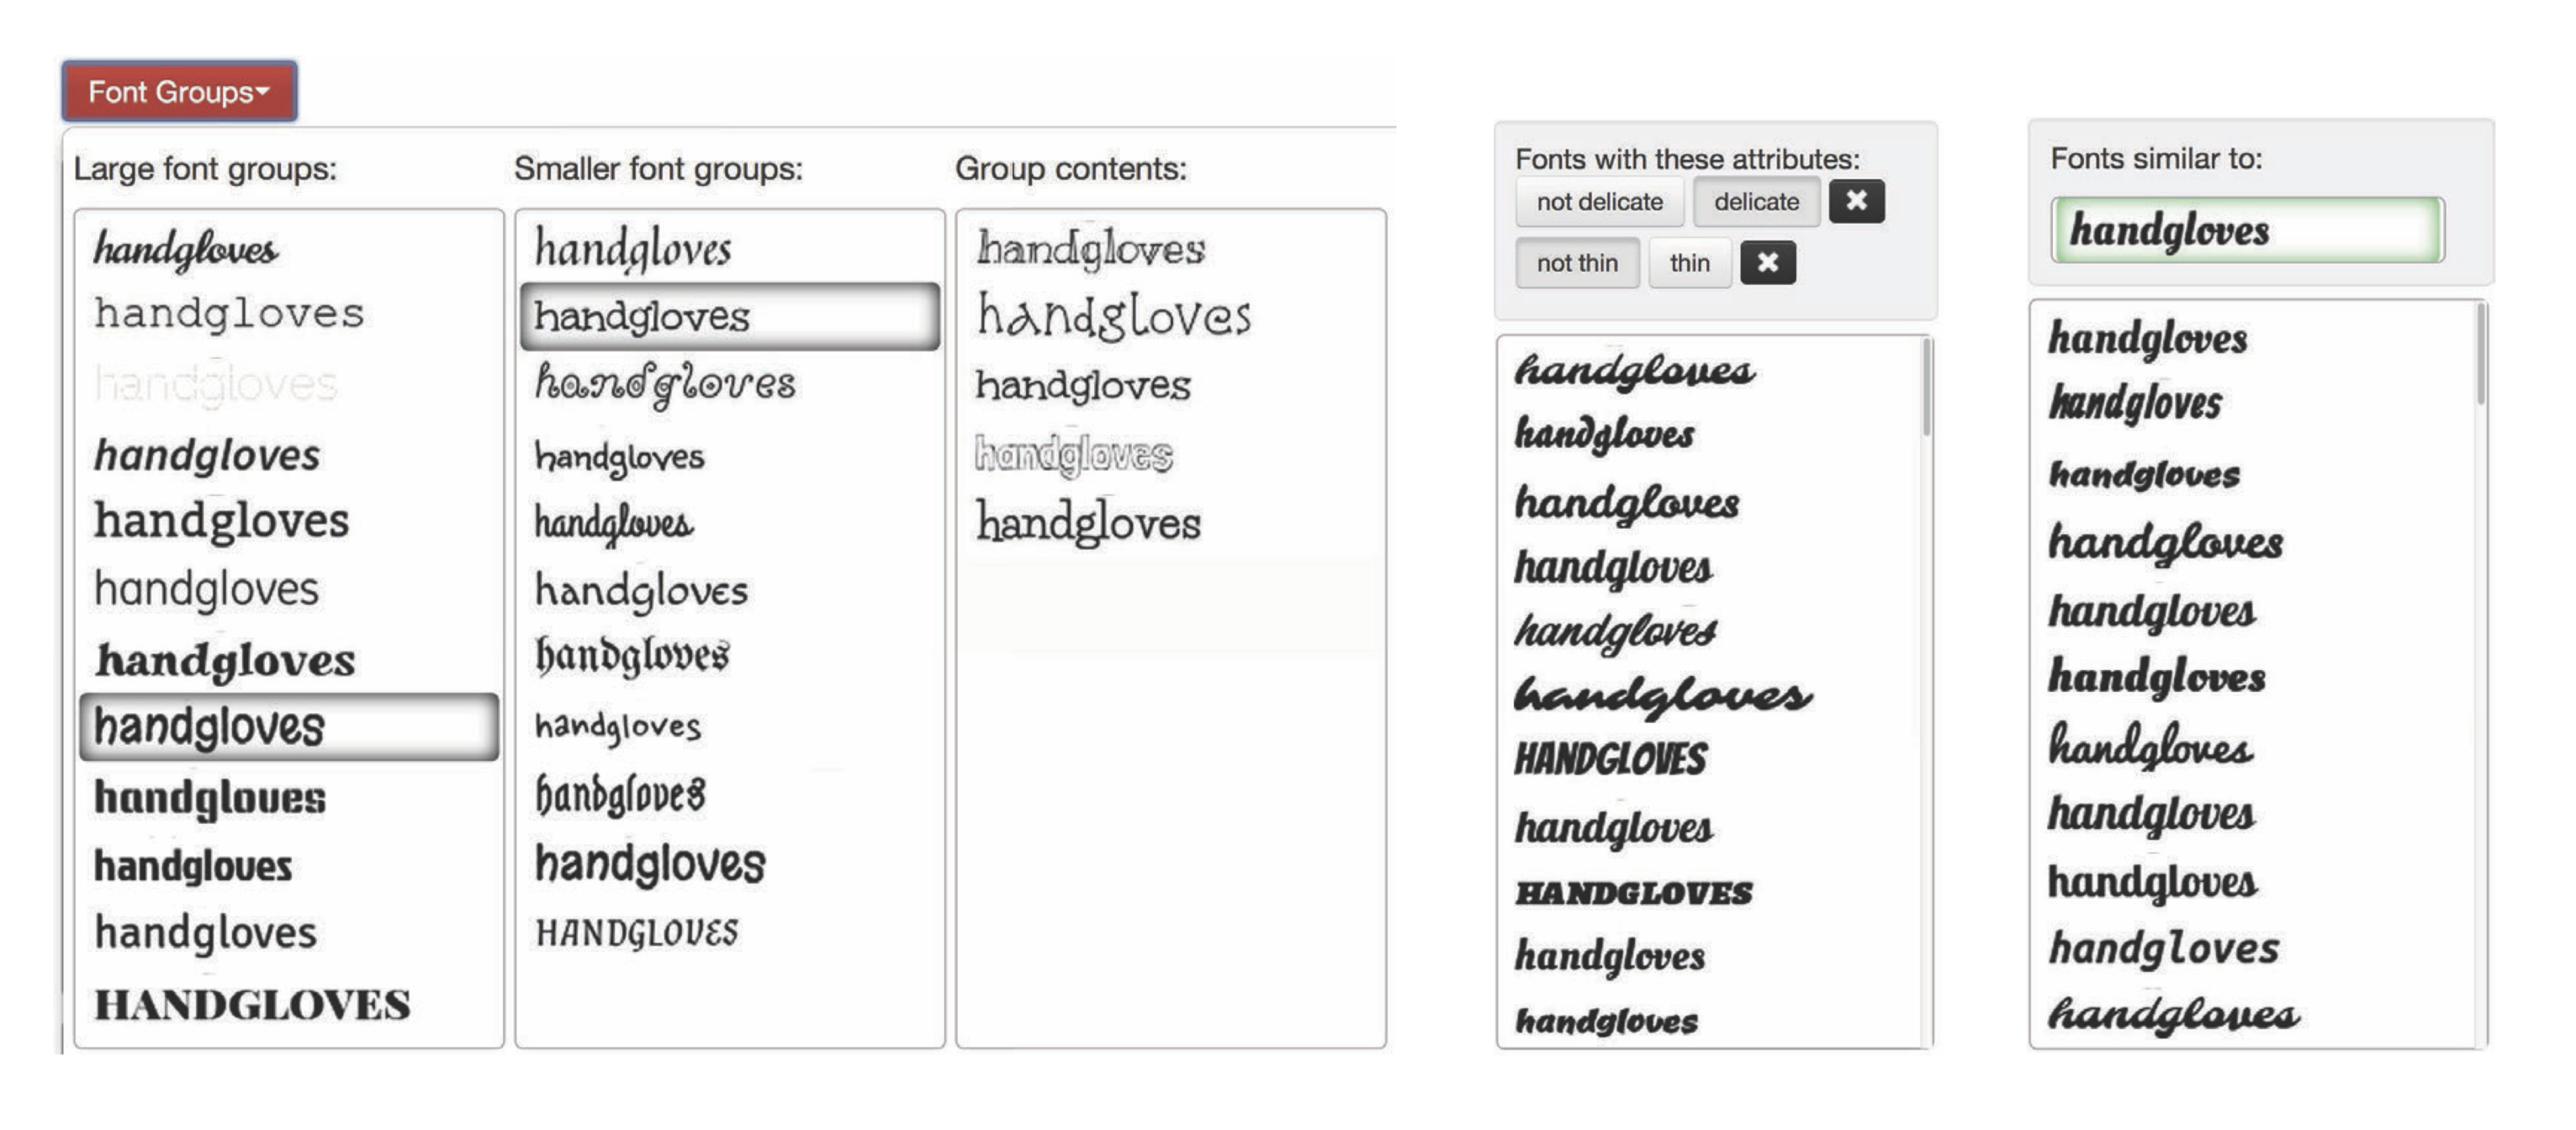
\includegraphics[width=1\textwidth]{images/odonovan-interfaces.png}
    \caption{Group Interface, Attribute Interface, and Search-By-Similarity selection tools from O'Donovan et al.}
    \label{fig:odonovan-interfaces}
\end{figure}

\section{Font Inference}

Besides O'Donovan et al. there has been a some effort to build inference models around font character images, often with the explicit purpose of building better user-interface for font selection. Cho et al. build a model with the explicit goal of generating latent space encodings of glyphs which are easily differentiable based on their font. They write:

\begin{quote}

For the discriminative representation of a font from others, we propose a paired-glyph
matching-based font representation learning model that attracts the representations of
glyphs in the same font to one another, but pushes away those of other fonts. \cite{cho2022}
	
\end{quote}

Their paired-glyph matching involves selecting random pairs of glyphs and training the model to prefer a low cosine similarity (more similar) between the representations if the glyphs are characters in the same font, and a high cosine similarity (less similar) if the glyphs come from different fonts.

\begin{figure}[h]
    \centering
    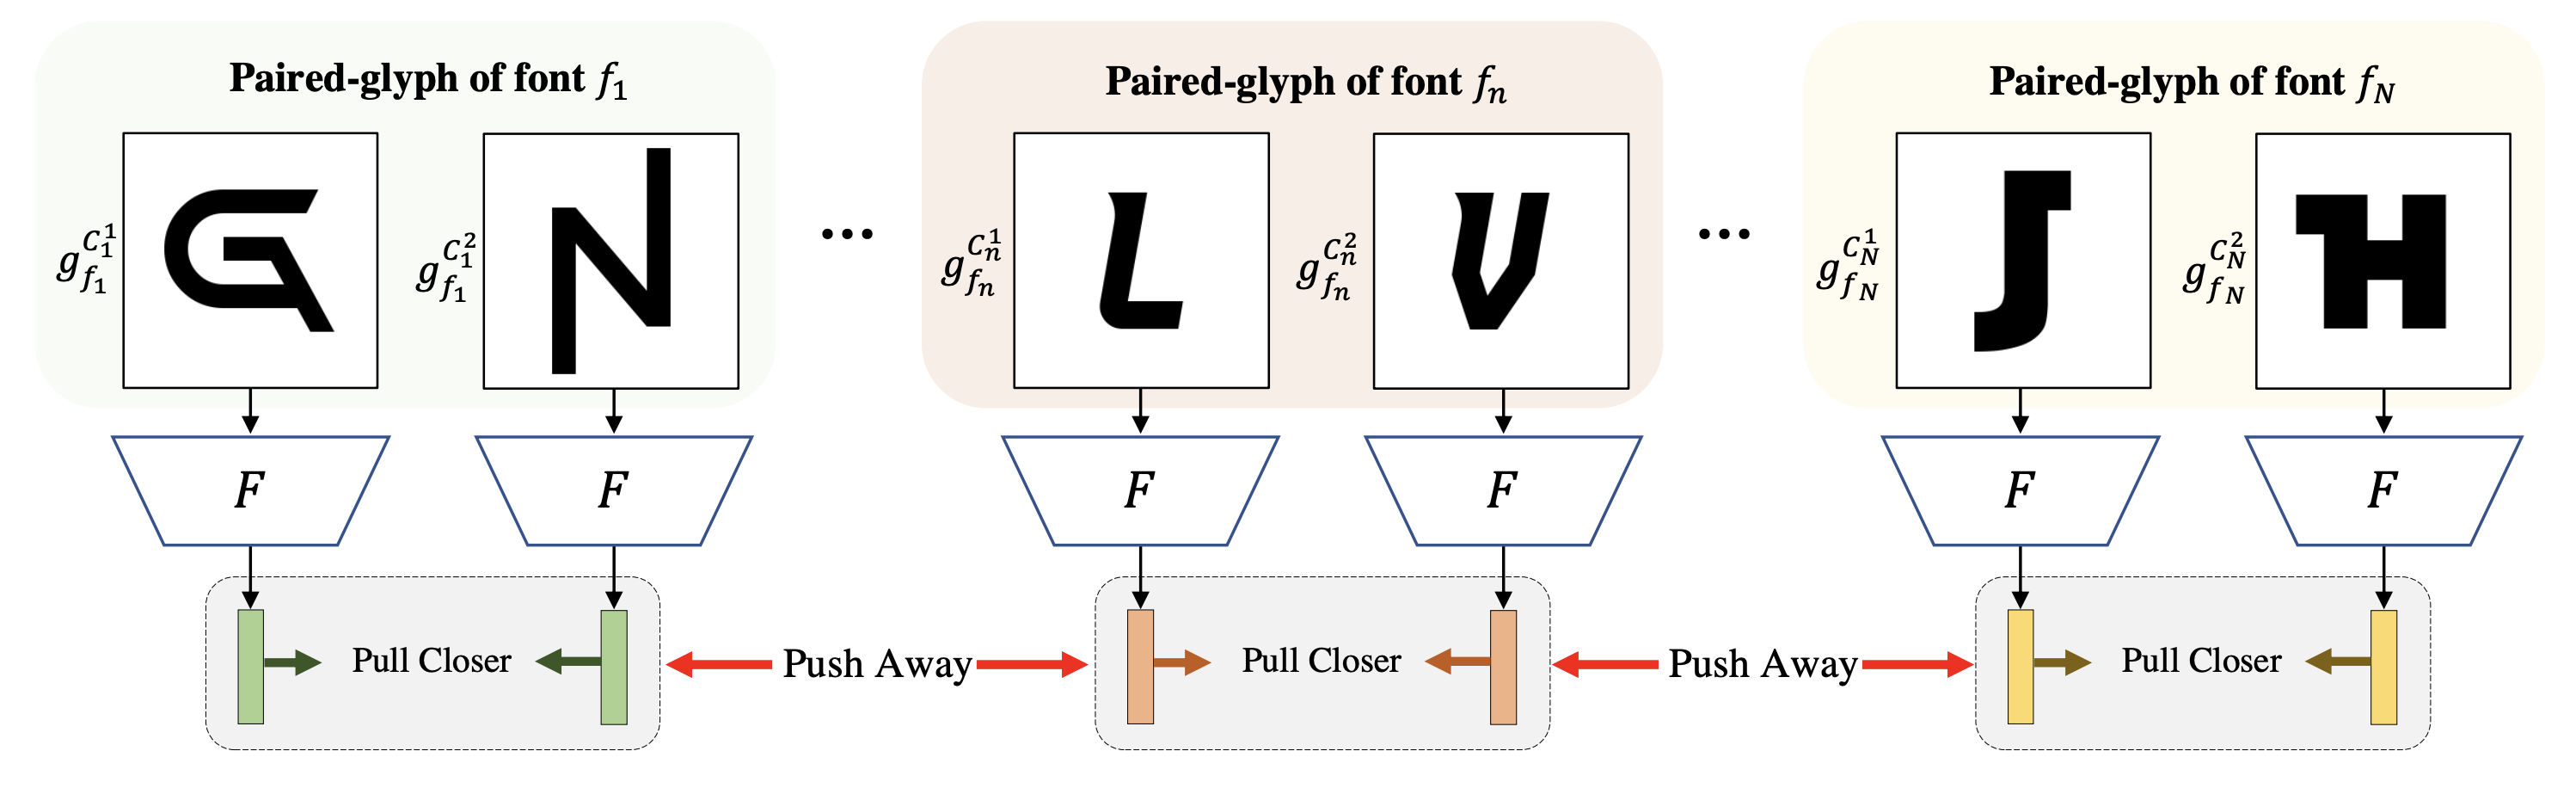
\includegraphics[width=1\textwidth]{images/cho-paired-glyph.png}
    \caption{Overall mechanism of paired-glyph matching in Cho et al.}
    \label{fig:cho-paired-glyph}
\end{figure}

Cho et al. succeed in their goal of clustering the latent space representations of glyphs by typeface, but likely because their evaluation prioritizes the same metric upon which the model is trained: latent space differentiation. They evaluate by determining whether, for a given input glyph, the correct font is chosen using closest-latent-space selection. Essentially, they are asking whether the model correctly encodes a glyph to its respective font. This is helpful in font discrimination, but it is unclear based on their results whether anything meaningful about the typefaces (style, weight, size) is encoded through their model.

\begin{figure}[h]
    \centering
    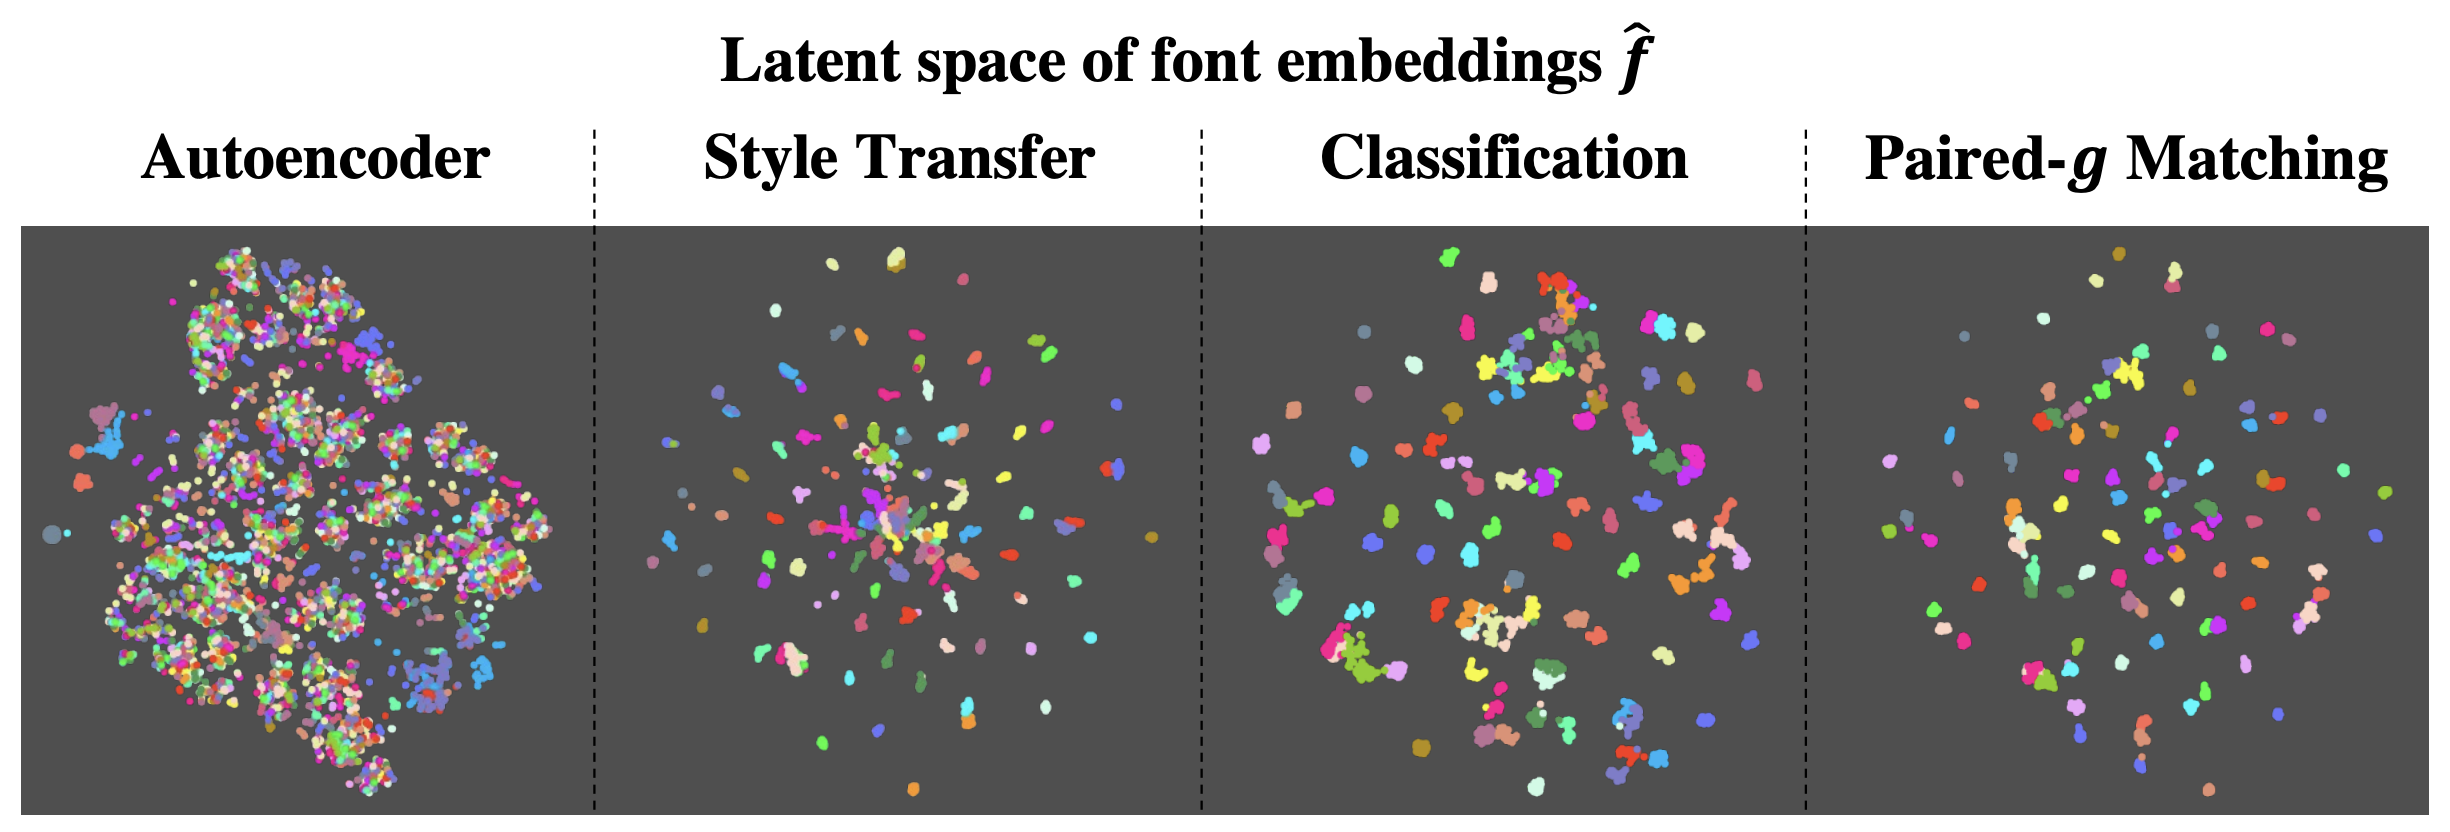
\includegraphics[width=1\textwidth]{images/cho-latent-space.png}
    \caption{Latent space of font embeddings given four different model techniques in Cho et al.}
    \label{fig:cho-latent-space}
\end{figure}

One aspect of Cho et al. which is helpful for our work is the set of model techniques which they tested. As shown in the latent space maps in Figure \ref{fig:cho-latent-space}, they employ three different model techniques, besides their paired-glyph matching, namely: autoencoding (training a model to recreate an input image), style transfer (generating another character in the same font given an input character), and classification (predicting which font is represented in a glyph). This supports our early choices to pursue autoencoder and style transfer models, and the latent space analysis is particularly useful in showing the effectiveness of these models' font encoding capacity.

Srivatsan et al. introduce an exciting novel training method in ``A Deep Factorization of Style and Structure in Fonts'' based on latent probability space and a tensor factorization approach well-founded in past literature \cite{srivatsan2020}. Their model explicitly seeks to disentangle style and content—to encode font style as separate from the actual character it represents. Their model, shown in Figure \ref{fig:srivatsan-model}, convolutionally encodes a probabilistic embedding of a subset of fonts given their complete character glyph set and corresponding character embeddings and uses that latent probability vector along with a given character embedding to reconstruct the glyph.

\begin{figure}[h]
    \centering
    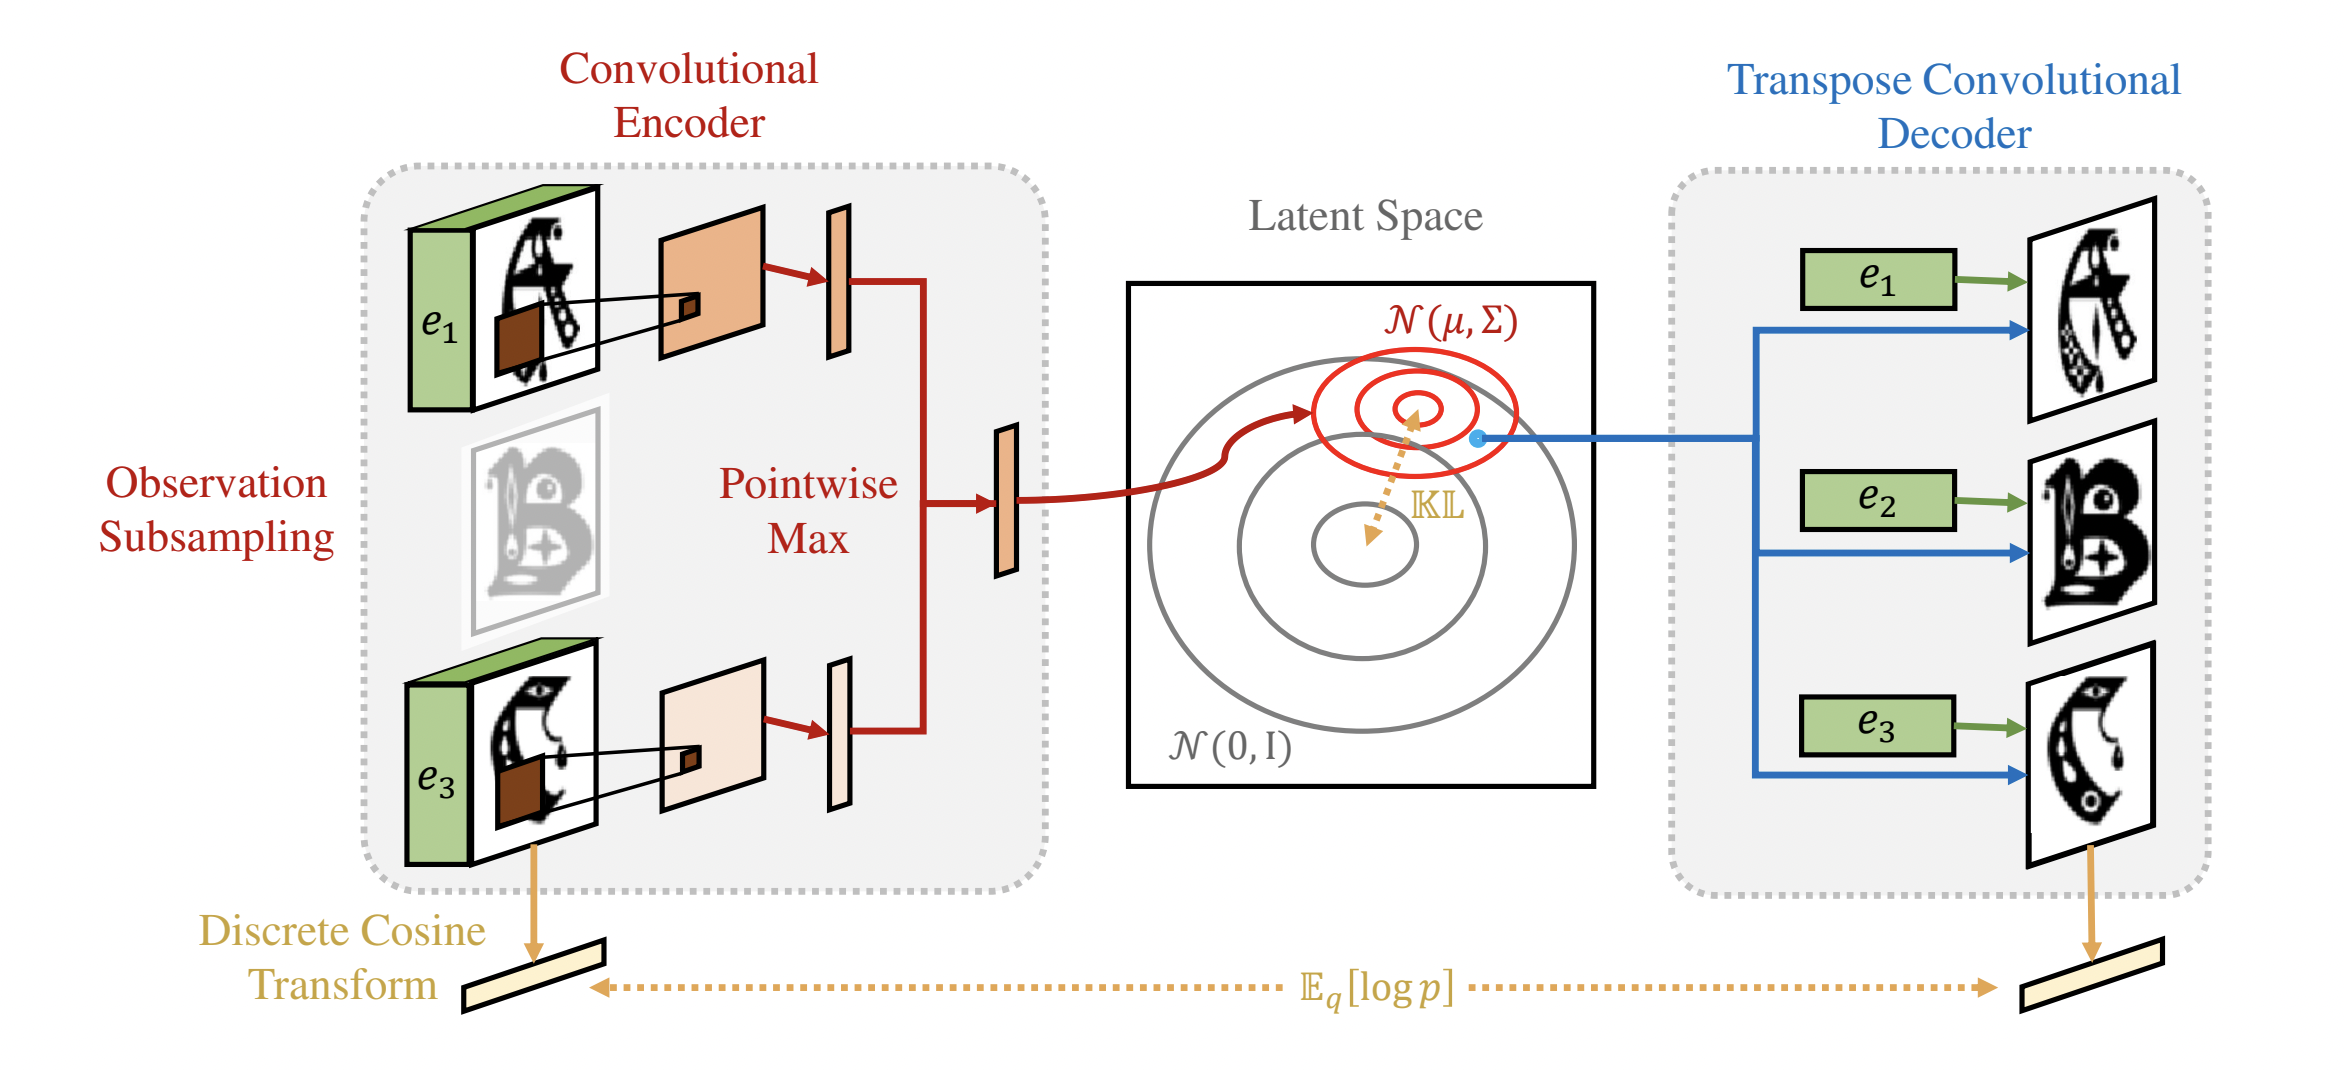
\includegraphics[width=.9\textwidth]{images/srivatsan-model.png}
    \caption{Generative process of model in Srivatsan et al.}
    \label{fig:srivatsan-model}
\end{figure}

At testing time, the model is given a certain number of glyphs in an unseen font (they tested on 1, 2, 4, and 8 observed characters) and is tasked with reconstructing the full glyph set for the typeface. Their model is particularly effective at reconstructing glyphs, when compared to peer models, and it also succeeds against a state-of-the-art peer model when evaluated by humans on Amazon Mechanical Turk. Figure \ref{fig:srivatsan-latent} shows a t-SNE projection of their model latent space with ``A'' glyphs displayed at each centroid given k-means clustering ($k=10$), and the researchers qualitatively find that their model effectively recreates many important aspects of character style.

\begin{figure}[h]
    \centering
    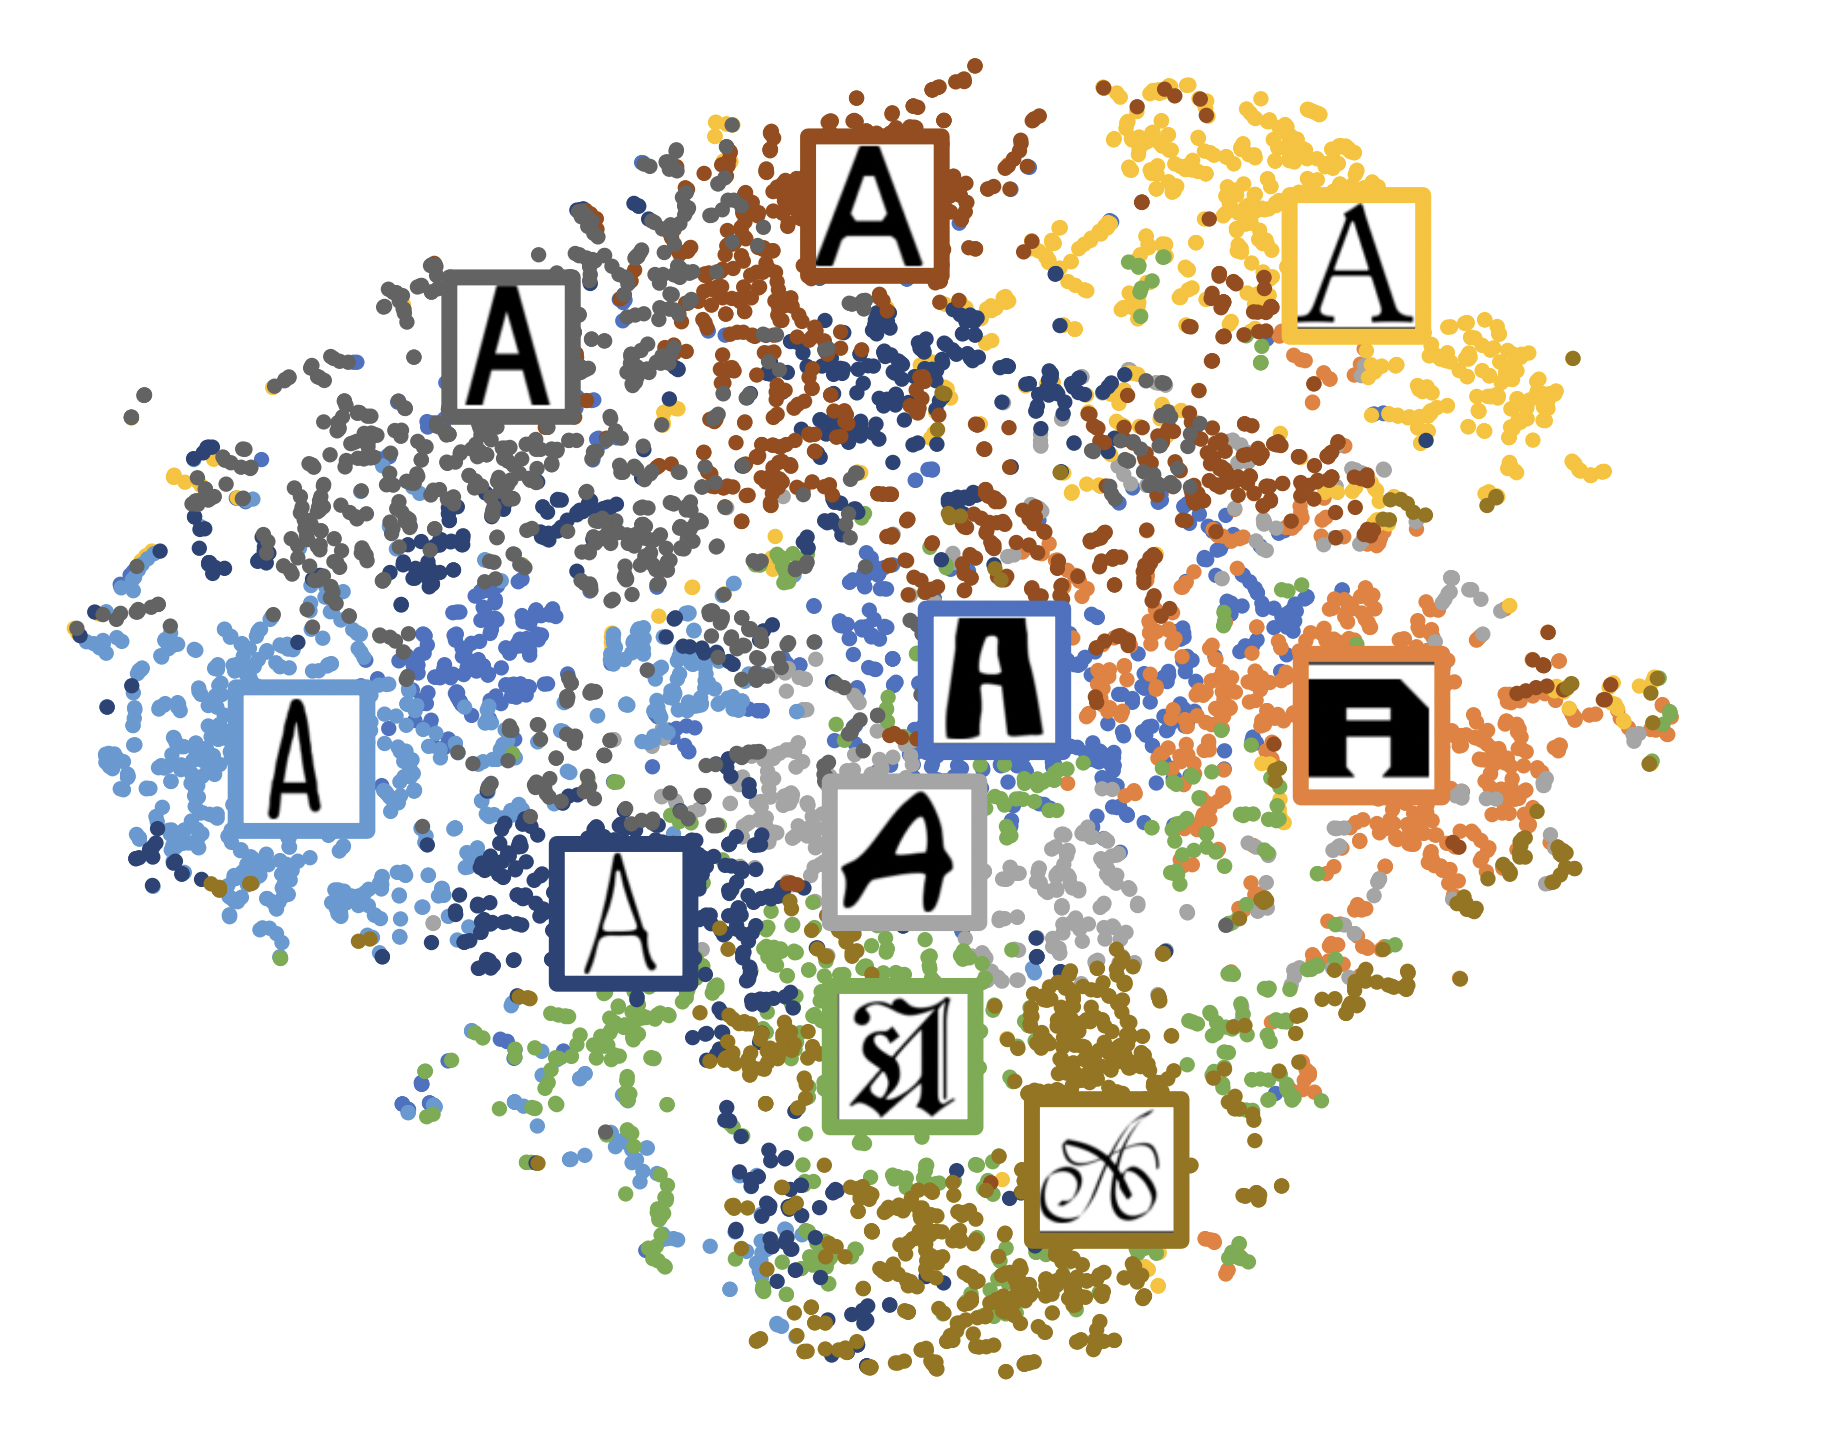
\includegraphics[width=.7\textwidth]{images/srivatsan-latent.png}
    \caption{t-SNE projection of latent font variables in Srivatsan et al., colored by k-means clustering ($k=10$) with ``A'' glyphs overlayed at each centroid.}
    \label{fig:srivatsan-latent}
\end{figure}
